\section{Introduction}

The term microbiome is used to refer to the collection of genes within a community of microbes (including bacteria, fungi, virus, protists and bacteriophages). In the last few years, microbiome research has helped us gained new insights into how microbes shape our human biology and have brought paradigm-shifting implications for translational research and clinical care. The human microbiota is crucial for our body to maintain its homeostasis. Disruption of this can lead to diseases such as obesity, inflammatory bowel disease, malnutrition, Parkinson's, Autism, Asthma, dental caries, bacterial vaginosis, and depression \cite{Knight2017}.  Currently, microbiome researchers use culture-independent techniques that involve DNA sequencing to derive the microbiome. Broadly, the community taxonomy/microbiome can be identified using two approaches (see Figure\ref{fig1}) 1) Targeted and 2) Metagenomic. Targeted sequencing approach uses the PCR amplified, target gene markers (16S rRNA in case of bacteria or ITS in case of Fungi) derived from the samples to reference it against gene-marker databases (Silva, Green Genes, etc.). In contrast, the metagenomic sequencing approach directly sequence the whole community DNA and compares it to reference genomes \cite{Morgan2012}.

\begin{figure}[ht]
	\centering
	\includegraphics[width=0.5\textwidth]{./image/introduction.png}
	\caption{A figure illustrating the different sequencing approaches used to derive the human microbiome, consisting of interacting bacteria, fungi and viruses. Adapted from: \cite{Morgan2012}}
	\label{fig1}
\end{figure}

Present microbiome studies focus on a single profile of the human microbiome in isolation, even though bacteria, fungi and viruses coexist and interact in the body as a community. Thus, it is essential to look at these biological components together in an integrated fashion to understand more holistically the true underlying in vivo state. However, one of the primary reasons for the lack of multi-biomic research is the lack of methods to merge microbiome datasets and integrative analysis. Consequently, I tried addressing some of these challenges in my master's thesis, using microbiome datasets derived from bronchiectasis patients as an example. Bronchiectasis, is a chronic inflammatory respiratory disease associated with progressive, irreversible dilatation of the airway. It is crucial to study bronchiectasis because in most cases it is known to be idiopathic(unknown cause) \cite{pmid29478908} and it is a significant contributor to lung diseases globally with a substantial four-fold higher predominance in Asian populations \cite{Seitz2012}. 

\begin{figure*}[!h]
	\centering
	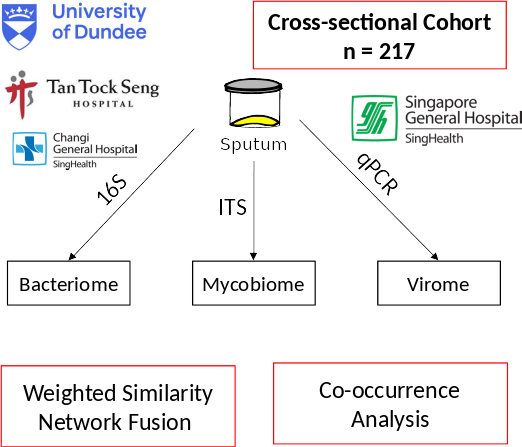
\includegraphics[width=0.50\textwidth]{./image/methods_masters.png}%
	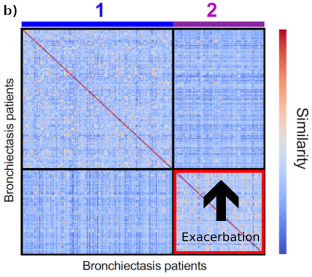
\includegraphics[width=0.50\textwidth]{./image/Res2.png}\\
	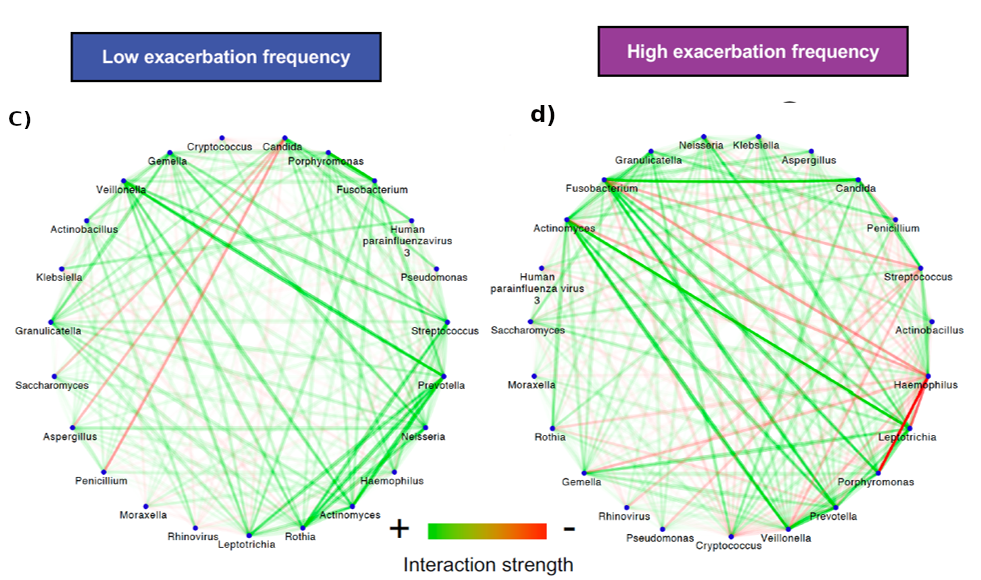
\includegraphics[width=\textwidth]{./image/Res3.png}
	\caption{(a) A schematic representing, overview of analysis performed on the CAMEB cohort (n=217). Methodologies: Weighted SNF and Co-occurrence analysis were used for microbiome integration and intreactome construction. (b) A patient similarity matrix with each cell representing the integrated similarity between patients. Two clusters of low (black) and high (red) risk patients identified by wSNF are highlighted by boxes. Visualization of the interactome of low (c) and high (d) risk clusters. Interactions between microbes are	classified as negative if the sign of the edge weights between them is negative (coloured red) with positive interactions indicated by green colouration. The strength of the interaction is indicated by the colour depth}
	\label{fig2}
\end{figure*}

Previously in my master's thesis, I developed weighted similarity network fusion (wSNF) to allow weightage of input datasets during integration, otherwise unaccounted by conventional SNF \cite{Wang2014}. Ensemble-based co-occurrence analysis strategy developed by Faust et al. \cite{Faust2012} was extended to allow weightage of individual methods in the ensemble along with other modification to better infer microbial association networks. Microbiome and Mycobiome derived using targeted amplicon sequencing of the 16S and ITS regions from the sputum samples of the CAMEB cohort \cite{Mac1800766}; virome from qPCR on an extensive panel of 17 respiratory viruses, were used as the example dataset to integrate the microbiomes (Figure\ref{fig2}a). Multi-biome (Microbiome, Mycobiome and Virome) integration by wSNF identifies a high-risk exacerbation cluster with increased precision (Figure\ref{fig2}b). Co-occurrence network analysis of this high-risk cluster revealed an elevated antagonistic interactome with reduced alpha-diversity (Figure\ref{fig2}c) \cite{Narayana2019}.

Having developed the wSNF and shown its increased precision to identify exacerbators (clinical outcomes); here in my PhD thesis, I attempt to extend my results further. I aim to develop a web tool to enable users to integrate their microbiome datasets and to illustrate its advantages using publicly available microbiome datasets. The tool would motivate clinicians and microbiome researchers to explore multi-biome strategies for their problem and aid them in integrating their datasets. Secondly, I aim to study exacerbation events, antimicrobial perturbations and ``Time to next exacerbation" using the developed ``Interactome" framework. Thirdly, I aim to validate the ``high-risk" exacerbation cluster of Bronchiectasis patients and its ``interactome" as derived in my previous work \cite{Narayana2019} using an alternate sequencing approach: metagenomics. Further, we also pick an interaction from the interactome of the high and low-risk clusters and validate it experimentally. 